% % % % % % % % % % % % % % % % % % % % % % 
% appendix.tex - Ian Huston
% 
% % % % % % % % % % % % % % % % % % % % % % 


% % % % % % % % % % % % % % % % % % % % % % % % % % % % % % % % 
% =========================================================== %
% % % % % % % % % % % % % % % % % % % % % % % % % % % % % % % %
\chapter{Appendix}
\label{ch:appendix}
% % % % % % % % % % % % % % % % % % % % % % % % % % % % % % % % 
% =========================================================== %
% % % % % % % % % % % % % % % % % % % % % % % % % % % % % % % %

The following materials supplement the calculations and discussions in the main thesis.

% % % % % % % % % % % % % % % % % % % % % % % % % % % % % % % % 
% =========================================================== %
% % % % % % % % % % % % % % % % % % % % % % % % % % % % % % % % 
\section{Analytic Solution of Generalised Sound Speed Relation}
\label{sec:apx-multi}
% % % % % % % % % % % % % % % % % % % % % % % % % % % % % % % % 
% =========================================================== %
% % % % % % % % % % % % % % % % % % % % % % % % % % % % % % % % 
\eq{eq:defalpha} can be analytically solved in full 
generality without imposing the limits (\ref{eq:Plimits}) on the 
derivatives of the kinetic function. This allows us to determine the 
most general class of models where the non-linearity parameter 
satisfies the condition $\fnleq \propto 1/\cs^2$ at leading order. 

In general \eq{eq:defalpha} takes the form 
% 
\begin{equation}
\label{eq:genPXeqn-multi}
(2-\alpha ) P_{,X}P_{,XX} + 4XP^2_{,XX} = \frac{2\alpha }{3}
X P_{,X}P_{,XXX}
\end{equation}
% 
and this reduces to 
% 
\begin{equation}
\label{eq:genreduce-multi}
\alpha \Upsilon_{,X} = (6-\alpha ) \Upsilon^2 + \frac{3(2-\alpha )}{2}
\frac{\Upsilon}{X} \, ,
\end{equation}
% 
where $\Upsilon \equiv P_{,XX}/P_{,X}$. 
\eq{eq:genreduce-multi} can be transformed into the 
linear equation
% 
\begin{equation}
\label{eq:lineargen-multi}
U_{,X}+ \frac{3(2-\alpha )}{2\alpha} \frac{U}{X} = \frac{\alpha -6}{\alpha}
\end{equation}
% 
after the change of variables $U \equiv 1/\Upsilon$
and the general solution to \eq{eq:lineargen-multi} is given by
%  
\begin{equation}
\label{eq:gensolnlinear-multi}
\frac{P_{,XX}}{P_{,X}} = \frac{1}{X\left[ f_2(\varphi) X^{(\alpha -6)/2\alpha}
-2 \right] } \, .
\end{equation}
% 
Integrating a second time implies that
% 
\begin{equation}
\label{eq:secondint-multi}
P_{,X} = -f_1 (\varphi ) \left( 1- f_2(\varphi ) X^{-s} \right)^{1/(2s)}  \, ,
\end{equation}
% 
where $s \equiv (\alpha -6 )/(2 \alpha)$ and we have redefined 
the arbitrary integration functions $f_i(\varphi )$.  
Finally \eq{eq:secondint-multi} can be formally integrated 
in terms of a hypergeometric function
%  
\begin{equation}
 \label{eq:thirdint-multi}
 P= -f_1X \,{_2}F_1 \left( -\frac{1}{s}, -\frac{1}{2s}; 1-\frac{1}{s}, f_2X^{-s}
\right)  \, ,
\end{equation}
%  
which represents the most general solution for this class of models. 
Note that we have set the
remaining constant of integration to zero to ensure 
that the kinetic function vanishes in the limit of
zero velocity. In fact this expression admits many 
different classes of solution, arising as limits
of the expansion of the hypergeometric function.


% The special case of $\alpha =2$ $(s=-1)$ implies (after a 
% further redefinition of the functions $f_i (\varphi ))$ that 
% % 
% \begin{equation}
% \label{eq:DBIsoln-multi}
% P = -f_1 \sqrt{1-f_2 X} -f_3
% \end{equation}
% % 
% and this corresponds to the standard DBI action (\ref{eq:DBIkinetic}) 
% \cite{chenetal,lidser2}.          


% % % % % % % % % % % % % % % % % % % % % % % % % % % % % % % % 
% =========================================================== %
% % % % % % % % % % % % % % % % % % % % % % % % % % % % % % % % 
\section{Generalised BM bound for Finite \texorpdfstring{$n$}{n} Models}
\label{sec:apx-genbmbound}
% % % % % % % % % % % % % % % % % % % % % % % % % % % % % % % % 
% =========================================================== %
% % % % % % % % % % % % % % % % % % % % % % % % % % % % % % % % 


For completeness we should also consider the 
BM bound \eqref{eq:genBMbound} for the finite $n$ multi-coincident brane models. This is
given by 
% 
\begin{equation}
\label{eq:BMAdS-multi}
r_* < -\frac{42}{N \Neff^2}\sqrt{1 +(n-1)^2Y}\fnleq \,,
\end{equation}
%  
and in the case of an $AdS_5 \times X_5$ throat simplifies to
%  
\begin{equation}
\label{eq:bmadsbound}
r_* < -\frac{5}{\Neff^2} 
\frac{\fnleq}{(n-1)\sqrt{N}} \,.
\end{equation}
%  
Comparing the limits in Eqs.~\eqref{eq:AdSupper-multi} and
\eqref{eq:bmadsbound} 
implies that the bound \eqref{eq:LHbound} is stronger than the corresponding BM
bound \eqref{eq:genBMbound} if 
% 
\begin{equation}
\label{eq:LHstrongerads}
n > 1 -5.5 \times 10^{-14} N^{3/2} \Neff^2 \fnleq \,,
\end{equation}
% 
and this condition is always satisfied if 
% 
\begin{equation}
\label{eq:allNbound-multi}
-5.5 \times 10^{-14} N^{3/2} \Neff^2 \fnleq  <1  \, .
\end{equation}
% 
Moreover, the bound \eqref{eq:allNbound-multi} will itself be satisfied for 
all values of $\fnleq$ and $N$ if it is satisfied when the limits 
$\fnleq =-151$ and $N=75852$ are imposed. Hence, we conclude that the bound
\eqref{eq:LHbound} 
is stronger for $\Neff < 75$. 
In general, it is difficult to quantify 
the magnitude of $\Neff$ without 
imposing further restrictions on the parameters of the models 
and, in particular, on the functional form of the inflaton potential. 
However, if the ratio $\varepsilon_H/P_{,X}$ remains approximately 
constant during the final stages of inflation, one would anticipate that 
$\Neff \lesssim 60$. Nevertheless, if $N \ll 75852$, the bound 
\eqref{eq:LHstrongerads} will only be violated for $n \le 3$ if 
$\Neff \gg 60$.


% % % % % % % % % % % % % % % % % % % % % % % % % % % % % % % % 
% =========================================================== %
% % % % % % % % % % % % % % % % % % % % % % % % % % % % % % % % 
\section{Analytic tests for \texorpdfstring{$\B,\wt{\C}$ and $\wt{\D}$}{B, C and D} terms}
\label{sec:apx-codetests}
% % % % % % % % % % % % % % % % % % % % % % % % % % % % % % % % 
% =========================================================== %
% % % % % % % % % % % % % % % % % % % % % % % % % % % % % % % % 

% 
% 
% Bterm
Analytic solutions can also be found for the $\B$, $\wt{\C}$ and $\wt{\D}$ terms.
The $\B$ term integral, $I_\B$, is given by
% 
\begin{align}
 \label{eq:bintegral-num}
I_\B &= 2\pi \int_{\kmin}^{\kmax} \d q\, q^2\dvp1(\qvi)\B(\kvi,\qvi) \nonumber\\
% 
     &= 2\pi\alpha^2 \int_{\kmin}^{\kmax} \d q\, q^{\frac{3}{2}}
\int_{0}^{\pi} \d\theta\, (k^2 + q^2 -2k q \cos{\theta})^{-1/4}
\cos{\theta}\sin{\theta}\,,
\end{align}
% 
and has the following analytic solution when $\dvp1(q) = \alpha/\sqrt{q}$:
% 
\begin{align}
\label{eq:intb-soln-num}
 I_\B = -\frac{\pi\alpha^2}{168 k^2}\Bigg\{ 
        &-63 k^4 \Bigg[ \log\Biggl(\frac{\sqrt{k}}{\sqrt{k+\kmin} + \sqrt{\kmin}}
                            \Biggr)
         + \log\Biggl( \frac{\sqrt{k+\kmax} +\sqrt{\kmax}}{\sqrt{\kmax-k} +
                      \sqrt{\kmax}}\Biggr) \nonumber \\
        &-\frac{\pi}{2} + \arctan\left( \frac{\sqrt{\kmin}}{\sqrt{k-\kmin}}\right)
        \Bigg] \nonumber\\
% 
        &+\sqrt{\kmax}\Bigg[ \left(-65k^3 + 8k\kmax^2 \right)\left(\sqrt{k+\kmax} +
          \sqrt{\kmax-k}\right) \nonumber \\
        &\qquad +\left(22k^2\kmax -16\kmax^3\right) \left(\sqrt{k+\kmax} -
         \sqrt{\kmax -k} \right) \Bigg] \nonumber \\
        &+\sqrt{\kmin}\Bigg[ \left(65k^3 - 8k\kmin^2 \right)\left(\sqrt{k+\kmin} -
          \sqrt{k-\kmin}\right) \nonumber \\
        &\qquad +\left(-22k^2\kmin +16\kmin^3\right) \left(\sqrt{k+\kmin} +
         \sqrt{k-\kmin} \right) \Bigg] \Bigg\} \,.
\end{align}
% 
If, in addition to $\dvp1(q) = \alpha/\sqrt{q}$, we also take
% 
\begin{equation}
 \dN{\dvp1}(q) = -\frac{\alpha}{\sqrt{q}} -i\frac{\alpha\sqrt{q}}{\beta}\,
\end{equation}
% 
then the $\wt{\C}$ and $\wt{\D}$ terms can be integrated analytically.
The integral of the $\wt{\C}$ term is 
% 
\begin{align}
 \label{eq:cint-num}
I_{\wt{\C}} &= \int\d^3 q\, \dvp1(\qvi) \dN{\dvp1}(\kvi-\qvi) 
    = 2\pi \int \d q\, q^2 \dvp1(\qvi) \wt{\C}(\kvi, \qvi) \nonumber\\
% 
 &= -2\pi\alpha^2 \int_{\kmin}^{\kmax} \d q\, q^{\frac{3}{2}} \int_0^\pi 
     \left( \left(k^2 + q^2 -2kq \cos\theta\right)^{-\frac{1}{4}} \right.\nonumber \\
            &\qquad \qquad \left.+\frac{i}{\beta}\left(k^2 + q^2 -2kq
\cos\theta\right)^{\frac{1}{4}}
        \right) \sin\theta \d \theta\,,
\end{align}
% 
and the analytic solution is given by
% 
\begin{align}
\label{eq:cint-soln-num}
I_{\wt{\C}} = -I_\A -i\frac{\pi\alpha^2}{240 \beta k}\Bigg\{ 
        &15 k^4 \Bigg[ \log\Biggl(\frac{\sqrt{k+\kmin} + \sqrt{\kmin}}{\sqrt{k}}
                            \Biggr)
         + \log\Biggl( \frac{\sqrt{\kmax-k} + \sqrt{\kmax}}{\sqrt{k+\kmax}
                        +\sqrt{\kmax}}\Biggr) \nonumber \\
        &-\frac{\pi}{2} + \arctan\left( \frac{\sqrt{\kmin}}{\sqrt{k-\kmin}}\right)
        \Bigg] \nonumber\\
% 
        &+\sqrt{\kmax}\Bigg[ \left(15k^3 + 136k\kmax^2 \right)\left(\sqrt{k+\kmax} +
          \sqrt{\kmax-k}\right) \nonumber \\
        &\qquad +\left(118k^2\kmax -48\kmax^3\right) \left(\sqrt{k+\kmax} -
         \sqrt{\kmax -k} \right) \Bigg] \nonumber \\
% 
        &-\sqrt{\kmin}\Bigg[ \left(15k^3 + 136k\kmin^2 \right)\left(\sqrt{k+\kmin} +
          \sqrt{k-\kmin}\right) \nonumber \\
        &\qquad +\left(118k^2\kmin +48\kmin^3\right) \left(\sqrt{k+\kmin} -
         \sqrt{k-\kmin} \right) \Bigg] \Bigg\} \,.
\end{align}
 % 
The integral of the $\wt{\D}$ term is 
% 
\begin{align}
 \label{eq:dint-num}
I_{\wt{\D}} &= 2\pi \int \d q\, q^2 \dvp1(\qvi) \wt{\D}(\kvi, \qvi) \\
% 
 &= -2\pi\alpha^2 \int_{\kmin}^{\kmax} \d q\, q^{\frac{3}{2}} \int_0^\pi 
     \left( \left(k^2 + q^2 -2kq \cos\theta\right)^{-\frac{1}{4}} \right.\nonumber\\
% 
        &\qquad\qquad\left.+\frac{i}{\beta}\left(k^2 + q^2 -2kq
\cos\theta\right)^{\frac{1}{4}}
        \right) \cos\theta\sin\theta \d \theta\,,
\end{align}
% 
and the analytic solution is
% 
\begin{align}
\label{eq:dint-soln-num}
I_{\wt{\D}} = -I_\B &-i\frac{\pi\alpha^2}{900\beta k^2}\Bigg\{ \nonumber \\
        &135 k^5 \Bigg[ \log\Biggl(\frac{\sqrt{\kmax-k} + \sqrt{\kmax}}{\sqrt{k}}
                            \Biggr)
         + \log\Biggl( \frac{\sqrt{k+\kmax} +\sqrt{\kmax}}{\sqrt{k+\kmin} +
                          \sqrt{\kmin}}\Biggr) \nonumber \\
        &\qquad -\frac{\pi}{2} + \arctan\left(
\frac{\sqrt{\kmin}}{\sqrt{k-\kmin}}\right)
        \Bigg] \nonumber\\
% 
        &-\sqrt{\kmax}\Bigg[ \left(-185k^4 + 168k^2\kmax^2-32\kmax^4
            \right)\left(\sqrt{k+\kmax} - \sqrt{\kmax-k}\right) \nonumber \\
        &\qquad +\left(70k^3\kmax +16k\kmax^3\right) \left(\sqrt{k+\kmax} +
         \sqrt{\kmax -k} \right) \Bigg] \nonumber \\
% 
        &+\sqrt{\kmin}\Bigg[ \left(-185k^4 + 168k^2\kmin^2 -32\kmax^4
            \right)\left(\sqrt{k+\kmin} - \sqrt{k-\kmin}\right) \nonumber \\
        &\qquad +\left(70k^3\kmin +16k\kmin^3\right) \left(\sqrt{k+\kmin} +
         \sqrt{k-\kmin} \right) \Bigg] \Bigg\} \,.
\end{align}
% 


% % % % % % % % % % % % % % % % % % % % % % % % % % % % % % % % 
% =========================================================== %
% % % % % % % % % % % % % % % % % % % % % % % % % % % % % % % % 
\section{Discussion of properties of source term for different potentials}
\label{sec:apx-srcdisc}
% % % % % % % % % % % % % % % % % % % % % % % % % % % % % % % % 
% =========================================================== %
% % % % % % % % % % % % % % % % % % % % % % % % % % % % % % % % 
The evolution of the source term for the four potentials has been discussed in
Section~\ref{sec:compare-res}, with particular emphasis on the evolution after horizon crossing as
shown in Figure~\ref{fig:cmp-src-kwmap}. Here the differences apparent at early times, shown in
Figure~\ref{fig:cmp-src-zoom-kwmap} are commented on.

At early times the first order perturbations are still very close to the Bunch-Davies initial
conditions as outlined in Section~\ref{sec:initconds-num}. In particular the perturbations are
highly oscillatory with phase $\exp(-k\eta)$, where $\eta$ is the conformal time. When
$\varepsilon_H$ is small this is given by 
% 
\begin{equation}
 \eta = -\frac{1}{aH(1-\varepsilon_H)}\,.
\end{equation}
% 
It is therefore instructive to plot the slow roll parameter $\varepsilon_H$ for the four potentials
at these early times, as has been done in Figures~\ref{fig:eps-apx} and \ref{fig:eps-zoom-apx}. For
completeness the other slow roll parameter $\eta_H$ defined in \eq{eq:etaHdefn-intro} has been
plotted in Figures~\ref{fig:eta-apx} and \ref{fig:eta-zoom-apx}. 

\begin{figure}
 \centering
 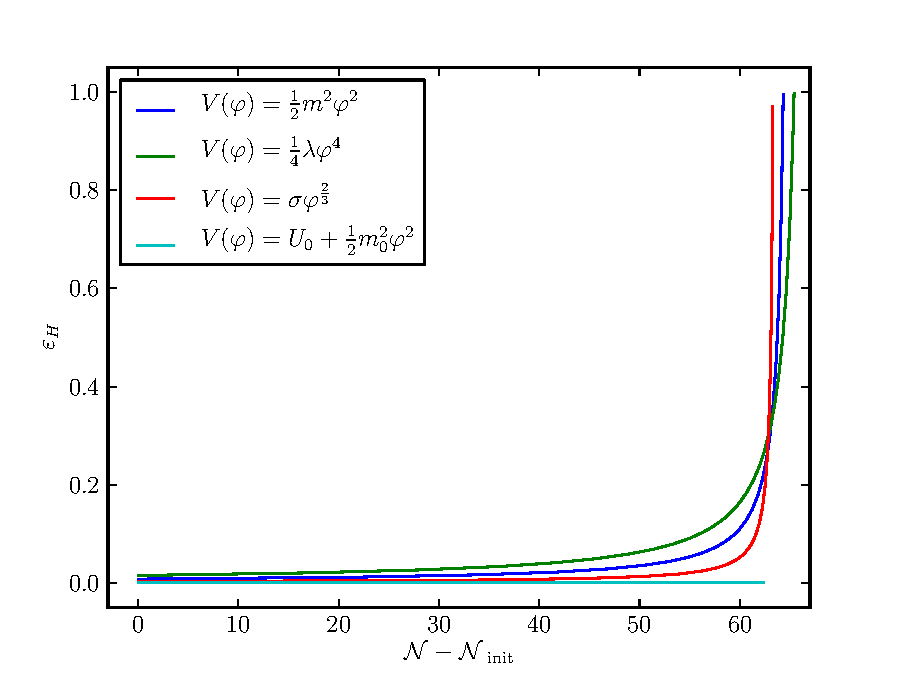
\includegraphics[width=0.75\textwidth]{numerical/graphs/epsilon_slowroll-large.pdf}
 % epsilon_slowroll-large.pdf: 432x324 pixel, 72dpi, 15.24x11.43 cm, bb=0 0 432 324
 \caption{The value of $\varepsilon_H$ for the four potentials.}
 \label{fig:eps-apx}
\end{figure}

\begin{figure}
 \centering
 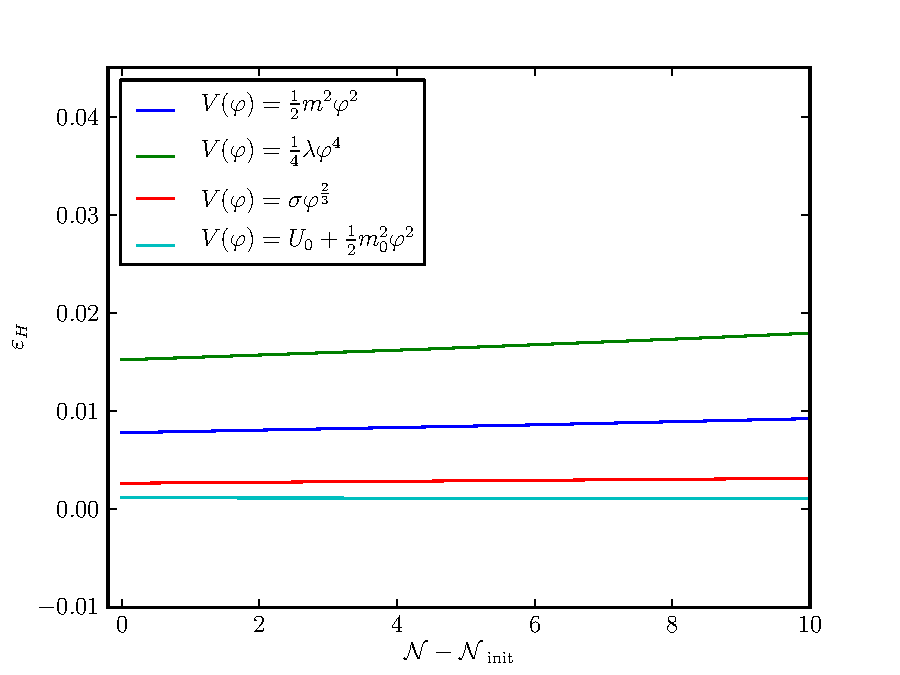
\includegraphics[width=0.75\textwidth]{numerical/graphs/epsilon_slowroll_zoom-large.pdf}
 % epsilon_slowroll-large.pdf: 432x324 pixel, 72dpi, 15.24x11.43 cm, bb=0 0 432 324
 \caption{The value of $\varepsilon_H$ for the four potentials at early times.}
 \label{fig:eps-zoom-apx}
\end{figure}

Figures~\ref{fig:eps-apx} and \ref{fig:eta-apx} show $\varepsilon_H$ and $\eta_H$ for the
four different models. Figures~\ref{fig:eps-zoom-apx} and
\ref{fig:eta-zoom-apx} show the early stages of the evolution as in
Fig~\ref{fig:cmp-src-zoom-kwmap}.

As is clear from these figures the change in the slow roll parameters is not easily related
to the differences in the profiles of the four potentials in Figure~\ref{fig:cmp-src-zoom-kwmap}. In
particular, although $\varepsilon_H$ and $\eta_H$ are quite different for the quadratic and quartic
models, the magnitude of $S$ after horizon crossing for these models is very similar.
\begin{figure}
 \centering
 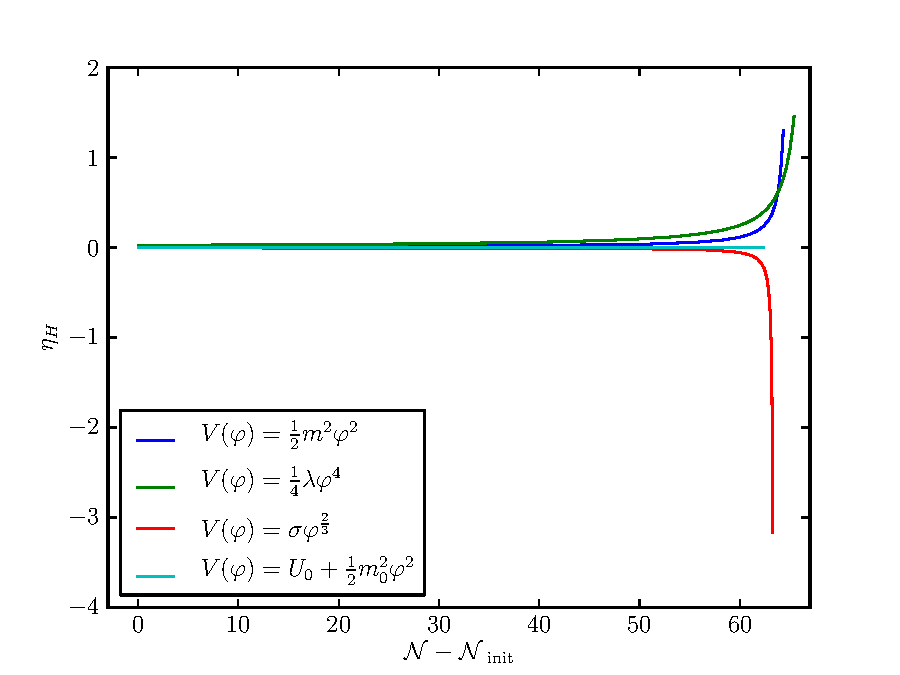
\includegraphics[width=0.75\textwidth]{numerical/graphs/eta_slowroll-large.pdf}
 % epsilon_slowroll-large.pdf: 432x324 pixel, 72dpi, 15.24x11.43 cm, bb=0 0 432 324
 \caption{The value of $\eta_H$ for the four potentials.}
 \label{fig:eta-apx}
\end{figure}

\begin{figure}
 \centering
 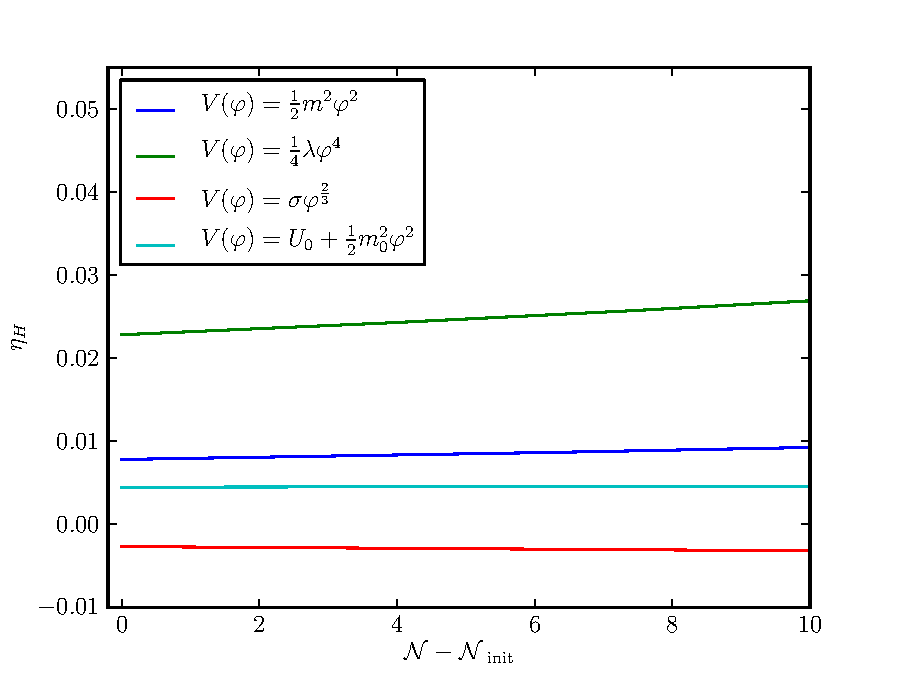
\includegraphics[width=0.75\textwidth]{numerical/graphs/eta_slowroll_zoom-large.pdf}
 % epsilon_slowroll-large.pdf: 432x324 pixel, 72dpi, 15.24x11.43 cm, bb=0 0 432 324
 \caption{The value of $\eta_H$ for the four potentials at early times.}
 \label{fig:eta-zoom-apx}
\end{figure}

At the earliest stages of the calculation of $S$, one or two e-foldings after the initialisation of
the first order perturbation, there appear to be small oscillations which affect the models in
different ways. The highly oscillatory initial conditions, combined with the small but appreciable
differences in $\varepsilon_H$ and $\eta_H$ contribute to this effect. In
Figure~\ref{fig:cos-keta-apx} the real part of the phase of the initial condition for $\dvp1$ is
plotted just after initialisation for the four potentials. The small differences in phase for each
model combined with the sharp cutoff at large and small $k$ values could explain the variations
in $|S|$ at early times as seen in Figure~\ref{fig:cmp-src-zoom-kwmap}. 

\begin{figure}
 \centering
 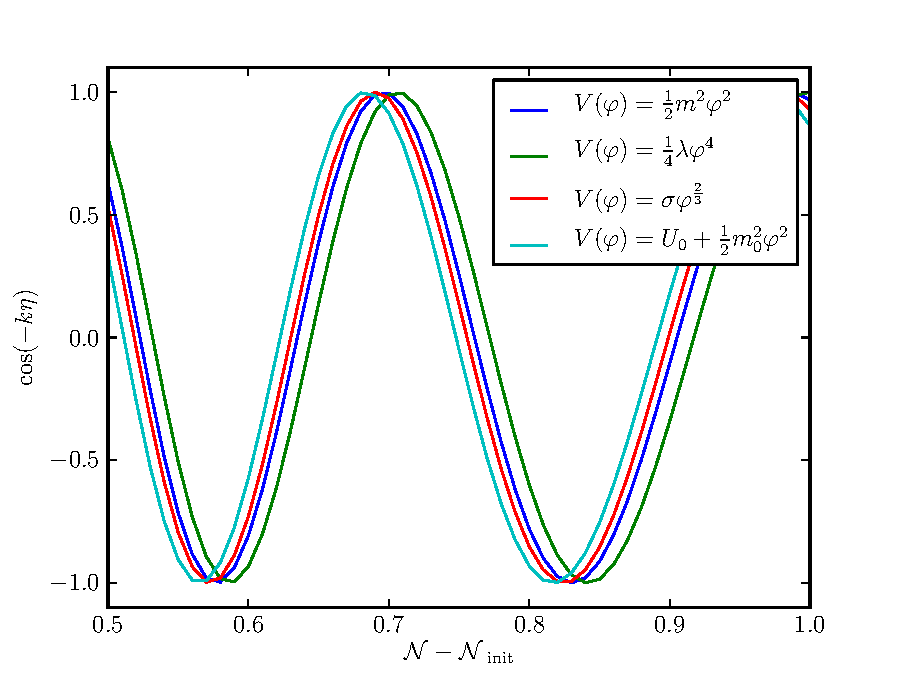
\includegraphics[width=0.75\textwidth]{numerical/graphs/cos_keta_kwmap_zoom-large.pdf}
 % cos_keta_kwmap_zoom-large.pdf: 432x324 pixel, 72dpi, 15.24x11.43 cm, bb=0 0 432 324
 \caption{The real part of the phase in the Bunch Davies initial conditions for the four different
potentials at early times.}
 \label{fig:cos-keta-apx}
\end{figure}
